\documentclass{beamer} % [aspectratio=169]
\usetheme{ucl}
\setbeamercolor{banner}{bg=darkred}
\setbeamersize{description width=2em}
\setbeamertemplate{navigation symbols}{\vspace{-2ex}} 

%\usepackage{fontspec}
\usepackage[utf8]{inputenc}
% \usepackage[english, greek]{babel}


\usepackage[T1]{fontenc} % Turn £ into $
\usepackage{minted}
\usemintedstyle{emacs}

\usepackage{fancyvrb}
\usepackage{xcolor}
\usepackage{url}

\usepackage{natbib}
\usepackage{bibentry}
\usepackage{url}


\usepackage{tikz}
\usetikzlibrary{positioning}



%\newcommand\emc[1]{\textcolor{brightblue}{\textbf{#1}}}
\newcommand\emc[1]{\textcolor{midred}{\textbf{#1}}}

\AtBeginSection[]{
  \begin{frame}
  \vfill
  \centering
  \begin{beamercolorbox}[sep=8pt,center,shadow=true,rounded=true]{title}
    \usebeamerfont{title}\insertsectionhead\par%
  \end{beamercolorbox}
  \vfill
  \end{frame}
}

\author{Mark Handley, University College London}
\title{About ENGF0002.}
\subtitle{Design and Professional Skills }
% \institute{}
\date{Term 1, 2018}


\begin{document}
\nobibliography*


\frame{
\titlepage
}

\begin{frame}
\frametitle{Notice of Recording \& Questions.}

This course is \emc{video recorded}, and your questions may be recorded too. 
\begin{itemize}
    \item Feel free to not provide your name in questions (I will not).
    \item We intend to make recordings available through moodle and lecture cast.
    \item We intend to upload the recordings to youtube for subtitling.
\end{itemize}

\vspace{3mm}
Please raise your hand at \emc{any time if you have a question}.
\begin{itemize}
    \item Ask for clarifications about the aims of teaching you anything.
    \item Or to help the understanding of the content of the course.
    \item Ask lecturers, and TAs, to speak slowly or write things down to help comprehension.
    \item More will follow \ldots
\end{itemize}

\end{frame} 


\begin{frame}
\frametitle{Welcome to UCL Engineering \& Computer Science!}

Our aim is to prepare you to be the \emc{best engineers in the world}!

\vspace{10mm}
Engineering is the discipline of \emc{shaping the world} around us 

for the \emc{benefit of humanity}.

\vspace{5mm}
\centering

\includegraphics[height=20mm]{img/internet.jpg} \quad
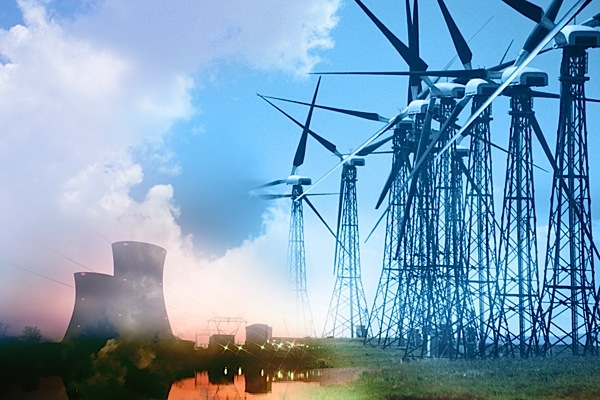
\includegraphics[height=20mm]{img/power.jpg} \quad
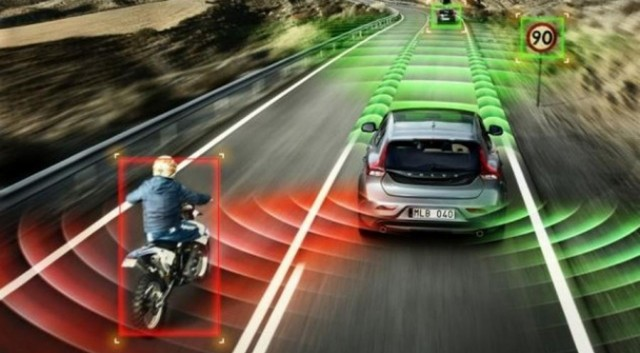
\includegraphics[height=20mm]{img/cars.jpg}

\end{frame}

\begin{frame}
\frametitle{The cost of bad engineering.}

Never forget the \emc{human cost} of bad engineering, 

and your \emc{personal professional responsibility}.

\vspace{10mm}
\centering
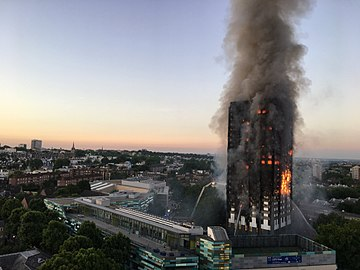
\includegraphics[height=23mm]{img/Grenfell.jpg} \quad
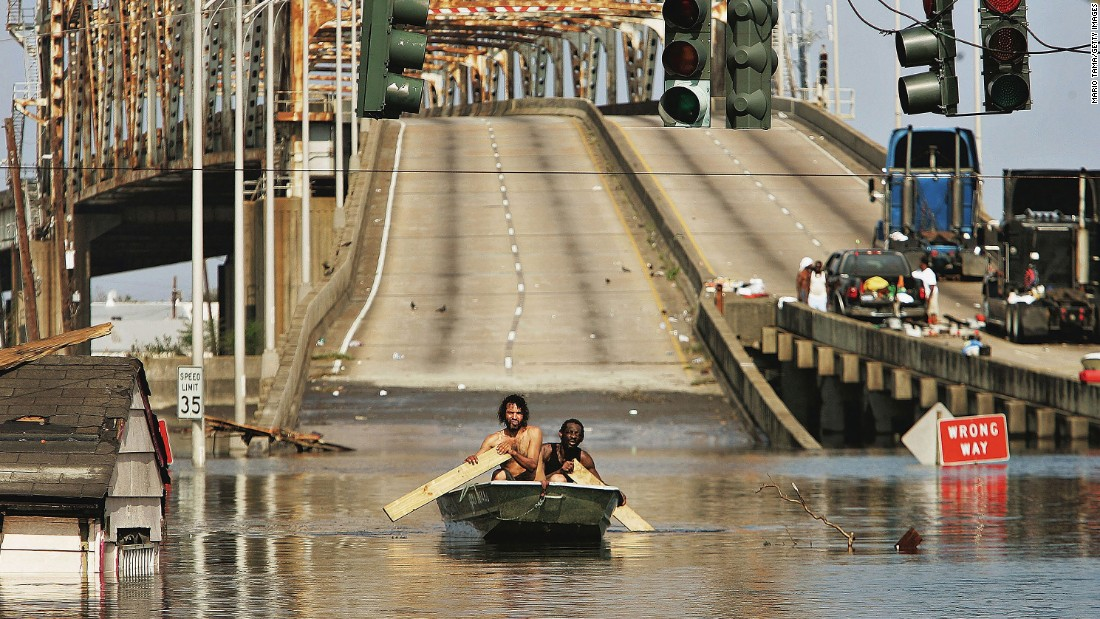
\includegraphics[height=23mm]{img/katrina.jpg} \quad
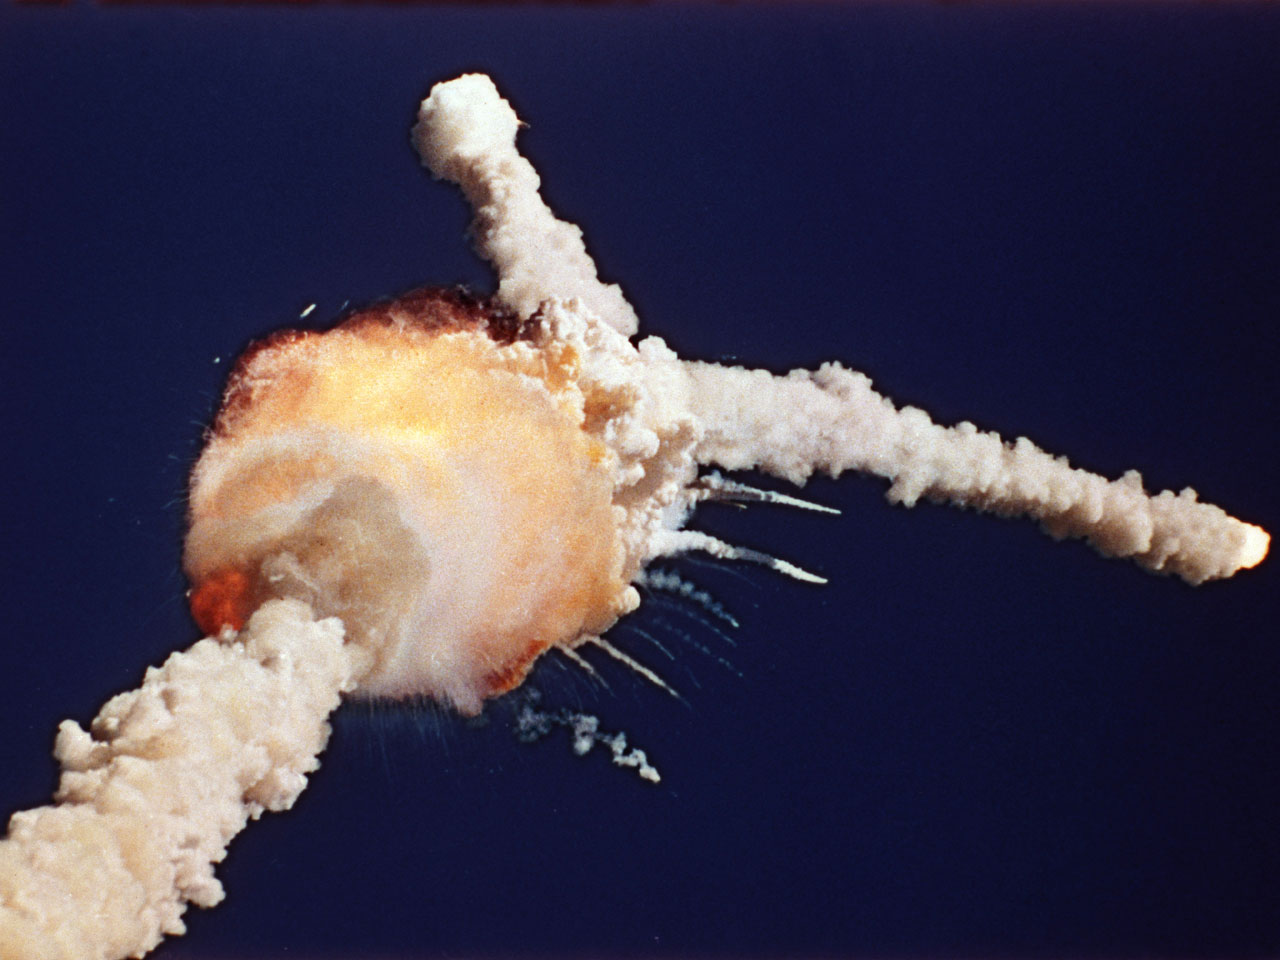
\includegraphics[height=23mm]{img/challenger.jpg}

\end{frame}

\begin{frame}
\frametitle{Overall aims of the ENGS102P.} 

The essence of good engineering is \emc{quality}. This course aims to:

\begin{itemize}
	\item Teach you professional skills important in all engineering.
	\item Teach you computer science specific professional skills.
	\item Expose you to important social and ethical discussions.
	\item Provide opportunities to practice all those skills.
\end{itemize}

\vspace{3mm} All teaching is by Computer Science faculty, but this is
an Engineering module, so some of the non-CS parts will be assessed by
Engineering staff.

\end{frame}

\begin{frame}
\frametitle{Who are we? The course leaders.} 

\begin{description}
\item[Mark Handley] is Professor of Networked Systems at UCL, with interests in Internet technologies, network protocols, and a bt of robotics.
\item[Stefano Vissicchio] is a Lecturer at UCL, with interests in in theory, algorithms and systems for efficiently and reliably managing communication networks.
\item[Matteo Sammartino] is a Researcher at UCL with interests in formal languages, coalgebras, process calculi, and automata learning.
\end{description}

\end{frame}

\begin{frame}
\frametitle{Who are we? Our teaching assistants.} 

\begin{description}
\item[Alberto Sonnino] is a Ph.D student in Security Engineering with a background in electrical engineering, information technologies and information security.
\item[Lisa Chalaguine] is a Ph.D student in Intellegent Systems that is working on chatbot technology for behaviour change, interested in machine learning, human-computer interaction and natural language processing. 
\item[Gerco Van Heerdt] is a Ph.D student in Programming Principles, Logic, and Verification who is interested in automata theory, category theory, and coalgebra.
\end{description}

\end{frame}


\begin{frame}
\frametitle{What Engineering Skills?} 

You will spend a significant part of your career \emc{communicating} with other engineers, other professionals and the public.

\vspace{3mm}
To help you we teach:
\begin{itemize}
\item Technical writing \& Technical argument.
\item Engineering visualization.
\item Technical Presentations.
\item Effective team work \& dynamics.
\end{itemize}
\end{frame}

\begin{frame}
\frametitle{What Computer Science Skills?} 

Computer Science lies at the intersection of \emc{mathematics} and \emc{engineering}. It solves problems through the manipulation of \emc{information}, and \emc{computation}.

\vspace{3mm}
This module will cover:
\begin{itemize}
	\item The \emc{principles of programming} illustrated in Python.
	\item Techniques for developing and reasoning about \emc{software correctness}.
	\item The principles of \emc{algorithms}, their implementation and performance.
	\item The organization of \emc{software production} in teams.
	\item Key tools and technologies for \emc{rapid prototyping}.
	\item Important \emc{social and ethical} dimensions of the information society.
\end{itemize}

\end{frame}

\begin{frame}
\frametitle{Topics Covered} 

\begin{center}
\begin{tabular}{ l l }
  \hline
  Computer Science & Engineering \\
  \hline
  Python Basics & Pebble in the Pond\\
  Debugging and Testing & Visualization\\
  Code Structure & Technical Argument\\
  Data Structures & Teamwork \\
  Algorithms & Technical Writing\\
  Development Practices & Presentation\\
  Networked Apps & Ethics\\
  Real-world Systems\\
  \hline
\end{tabular}
\end{center}
%% \begin{center}
%% \begin{tabular}{ c l l }
%% \hline 
%%  {\bf Week} & {\bf Tuesday} & {\bf Friday} \\ 
%% \hline 
%% W1  & Intro. \& Basics  & \emph{Pebble in the Pond}  \\  
%% W2  &  Basics & \emph{Visualisation} \\
%% W3  &  \emph{Technical Argument} & Data Struct. \& Algo.  \\
%% W4  &  Data Struct. \& Algo. & Dynamic Data Struct. \\
%% W5  & \emph{Writing} & \emph{Presentation} \\
%% W6  &  Dynamic Data Struct. & Develop. Practices \\
%% W7  &  Develop. Practices & \emph{Teamwork} \\
%% W8  &  Data \& Databases & Data \& Databases \\
%% W9  &  Networked Apps. & Networked Apps. \\
%% W10  & Real-world systems & Real-world systems \\
%%  \hline     
%% \end{tabular}
%% \end{center}

\end{frame}

\begin{frame}
\frametitle{Lectures} 

Familiarize your self with the timetable: \url{https://timetable.ucl.ac.uk}.

\begin{itemize}
\item Tuesday 09:00--11:00 -- Lectures.\\
Birkbeck Clore Management Centre B01
\item Friday 11:00--13:00 -- Lectures.\\
Anatomy G29 J Z Young LT
\end{itemize}
\end{frame}

\begin{frame}
  \frametitle{CS Practical Work}

  Aim is to have some practical work every week - most of it programming.

\vspace{3mm}
  Most of the practical exercises are \emc{not assessed}.  You must hand in
  a reasonable attempt at solution though - will receive a \emc{binary
  mark}.

 \begin{description}
  \item[{\bf For unassessed exercises,}] you may work with your friends, or in
  small groups.  You can learn a lot by discussing ideas together.

  \vspace{3mm}
Generally, working in pairs works best.  In larger groups you learn
  less.

  \item[{\bf For assessed excercises,}] your work \emc{\bf must be your own}.  We will make
  it clear which these are, and will run plagiarism detection software
  on the submissions.
  \end{description}
\end{frame}

\begin{frame}
  \frametitle{Practical Exercises}

  Goal is to learn by doing
  And by having some fun

  Will give you software for some simple retro games.
  Your tasks:
  \begin{enumerate}
  \item Play game, find bugs.
  \item Understand bugs by reading and instrumenting code.
  \item Fix the bugs.
  \end{enumerate}
  Option: improve the games.
\end{frame}

\begin{frame}
  \frametitle{Why Debugging?}

  \begin{itemize}
  \item You can't write bug free code.
  \item You can't write non-trivial code unless you can debug it.
  \item You can only learn debugging by doing it.
  \item Debugging trivial code doesn't teach you much.
  \end{itemize}

  Forces you to confront code that you don't understand, and
  progressively learn about it.
  \vspace{2mm}
  \begin{description}
  \item Teaches you programming by example.
  \item Teaches you about code structure.
  \end{description}
\end{frame}

\begin{frame}
  \frametitle{Assessment}

  Course has no exam.
  \begin{itemize}
    \item Binary marks from practical exercises and classroom tests 5\%.
    \item Mid-term coursework (week 5): 15\%
    \item Techical writing coursework (week 8): 15\%
    \item Ethics report (400-500 words, due end of Feb 2018): 15\%
    \item Ethics report presentations (during term 2 reading week): 10\%
    \item CS Scenario week (term 2): 40\%
  \end{itemize}

We will provide more information during term.

\end{frame}

\begin{frame}
\frametitle{Pebble in the Pond activity} 

Friday 5th October, 11am-1pm. Jeffery Hall.

\begin{itemize}
	\item You are working in groups of 5-6 (from ENGF0001).
	\item Each group is in charge of a segment of table.
	\item You are provided materials, and need to design a machine.
	\item That takes a pebble (rock) from one end of the set of tables to the other. The pebble must only touch the machine.
	\item Aims: fun, opportunity to meet \& reflections on team work.
\end{itemize}


Arrive promptly at 11am, find your group, and pick a CS table at random quickly! Then listen to the instructions carefully.

\vspace{0.24in}
2017 Taster: \url{https://mediacentral.ucl.ac.uk/Player/95966042}
\end{frame}

\begin{frame}
\frametitle{Course material.} 

All course material is available on-line, on github and moodle.

\vspace{7mm}
Computer Science specific \emc{syllabus, slides \& code}: 

\url{https://github.com/mhandley/ENGF0002}

\vspace{7mm}
To support you while learning the Python programming language:

\vspace{2mm}
Allen Downey. \emc{Think Python}. Green Tea Press. (free e-book)

{\small \url{http://greenteapress.com/thinkpython/thinkpython.pdf} }

\vspace{2mm}
Bruce Eckel. \emc{Thinking in Python}. (More advanced)

{\small \url{http://docs.linuxtone.org/ebooks/Python/Thinking_In_Python.pdf} }


\end{frame}

\begin{frame}
\frametitle{How to seek help with the course.} 

Use the Moodle discussion board first for questions: 
\url{https://moodle.ucl.ac.uk/course/view.php?id=43301&section=15}

\vspace{3mm}
Our excellent team of TAs help with questions and provide feedback:
\begin{itemize}
\item Alberto Sonnino --- \url{alberto.sonnino@cs.ucl.ac.uk}
\item Lisa Chalaguine --- \url{lisa.chalaguine.16@ucl.ac.uk}
\item Gerco Van Heerdt --- \url{gerco.heerdt.16@ucl.ac.uk}
\end{itemize}

We plan to run ENGF0002 programming clinics daily, whenever you have practical
exercises running.
\end{frame}

\begin{frame}
  \frametitle{Daily Programming Clinics.}

  Current plan:
  \begin{itemize}
  \item Monday, 3-5pm
  \item Tuesday, 11am-1pm
  \item Wednesday, 1-3pm
  \item Thursday, 11am-1pm
  \item Friday, 1-3pm
  \end{itemize}

  Malet Place Engineering Building, 7th floor lift lobby.

  No need to book, but if you all turn up at once, won't work.
\end{frame}

\begin{frame}
\frametitle{How to communicate issues about the course.}

We always welcome your feedback to improve courses!

\vspace{3mm}
Provide feedback and fixes to course material using the Github issue tracker:
\url{https://github.com/mhandley/ENGF0002/issues}

\vspace{3mm}
You are welcome to bring up any issues to:
\begin{itemize}
	\item the \emc{course leaders or TAs}.
	\item the \emc{1st year coordinator} (\url{J.Brotherston@ucl.ac.uk}).
	\item our Dept. \emc{teaching team} (\url{n.gosai@ucl.ac.uk}).
	\item the \emc{Director of Studies} (\url{L.Capra@cs.ucl.ac.uk}).
	\item the \emc{Head of Department} (\url{J.Shawe-Taylor@cs.ucl.ac.uk})
\end{itemize}

\end{frame}

\begin{frame}
\frametitle{Professionalism \& Code of Conduct (I).}

We expect you to keep a very high standard of \emc{professionalism} in this course. Including a high degree of \emc{courtesy} in all your interactions, and \emc{integrity} when it comes to assessment.

\vspace{3mm}
The \emc{British Computing Society} (BCS) defines a code of conduct:
\begin{description}
	\item[The Public interest]: Respect for public health, privacy, security and wellbeing of others and the environment. Respect the rights of others. Conduct activities without discrimination, and extend to all the benefits of computing.
	\item[Competence and Integrity]: do not overclaim your competence, and only accept work within it; keep up professional development; respect all view points and offer honest opinions; do not be malicious or neglectful; do not bride or be bribed.
\end{description}

\end{frame}

\begin{frame}
\frametitle{Professionalism \& Code of Conduct (II).}

\begin{description}
	\item[Duty to Relevant Authority]: Implement diligently requirements, while exercising your judgment; avoid conflicts of interest; accept personal responsibility for your work and reports; keep confidences; and do not withhold relevant information.
	\item[Duty to the profession]: improve standards in the profession; support the BCS activities and members, and do not bring it into disrepute.
\end{description}

\vspace{3mm}
Full code of conduct: \url{http://www.bcs.org/category/6030}.

\vspace{3mm}
If ever in doubt please approach us for discussion or advice.

\end{frame}


% ---------------------------------

\bibliographystyle{alpha}
\nobibliography{references}

\end{document}
